\section{94 - AN 4.2, FA 6.4, FA 6.3, FA 6.2, AG-L 4.4 - Überlagerung von Schwingungen - Matura - 1. NT 2017/18}

\begin{langesbeispiel} \item[1] %PUNKTE DES BEISPIELS
Ein Ton in der Musik kann im einfachsten Fall durch eine Sinusfunktion $s$ mit $s(t)=a\cdot\sin(b\cdot t)$ für $a,b\in\mathbb{R}^+$ beschrieben werden. Bei einer derartigen Sinusschwingung wird der maximale Funktionswert als Amplitude bezeichnet. Die Anzahl der Schwingungen pro Sekunde wird als Frequenz $f$ bezeichnet und in Herzt $(Hz)$ angegeben.\\
Für die Frequenz $f$ gilt: $f0\frac{1}{T}$ (mit $T$ in Sekunden), wobei $T$ die (kleinste) Periodenlänge der jeweiligen Sinusschwingung ist $(T\in\mathbb{R}^+)$.

Drei bestimmte Töne werden mithilfe der nachstehenden Funktionen $h_1, h_2$ und $h_3$ beschrieben.\\
Die Zeit $t$ $(t\geq 0)$ wird dabei in Millisekunden (ms) gemessen.

$h_1(t)=\sin(2\cdot\pi\cdot t)$\\
$h_2(t)=\sin(2,5\cdot\pi\cdot t)$\\
$h_3(t)=\sin(3\cdot\pi\cdot t)$

Die Überlagerung mehrerer Töne bezeichnet man als Klang.\\
Die Funktion $h$ mit $h(t)=h_1(t)+h_2(t)+h_3(t)$ beschreibt einen Klang.

Der Schalldruck eines Tons ist zeitabhängig und kann durch die Funktion $\rho$ mit $\rho(t)=\bar{\rho}\cdot\sin(\omega\cdot t)$ beschrieben werden. Dabei sind $\bar{\rho}$ und $\omega$ Konstanten.\\
Der Schalldruck wird in der Einheit Pascal (Pa) angegeben.


\subsection{Aufgabenstellung:}
\begin{enumerate}
	\item Gib für einen Ton, der mithilfe der Funktion $g$ mit $g(t)=\sin(c\cdot\pi\cdot t)$ mit $c\in\mathbb{R}^+$ und $t$ in ms beschrieben wird, eine Formel für die Periodenlänge $T$ (in ms) in Abhängigkeit von $c$ an!
		
		Der Effektivwert $\rho_{\text{eff}}$ des Schalldrucks einer Sinusschwingung mit der Periodenlänge $T$ (in ms) kann mit der Formel $\rho_{\text{eff}}=\sqrt{\dfrac{1}{T}\displaystyle\int^T_0{\rho^2(t)}\,\text{d}t}$ berechnet werden.
		
		Berechne den Effektivwert des Schalldrucks eines Tons, wenn $\bar{\rho}=1$ und $\omega=2\cdot\pi$ gilt!
		
		\item Gib (z.B. unter Zuhilfenahme eines geeigneten Graphen) die (kleinste) Periodenlänge $T$ (in ms) der Funktion $h$ an!
		
		Gib die Frequenz $f$ der Funktion $h$ in Hertz an!
		
		\item Gib (z.B. unter Zuhilfenahme eines geeigneten Graphen) die Amplitude der Funktion $h$ und denjenigen Zeitpunkt $t\geq 0$ (in ms) an, zu dem die Amplitude erstmals erreicht wird!
		
		Begründe, warum die Amplitude von $h$ nicht gleich der Summe der drei Amplituden der Funktionen $h_1, h_2$ und $h_3$ ist!
		
		\item Für ein angenehmes Raumklangerlebnis (z.B. in einem Heimkino) ist es günstig, wenn die fünf Lautsprecher eines Fünf-Kanal-Tonsystems wie in nachstehender linker Skizze dargestellt angeordnet sind (Ansicht von oben). Vereinfach kann die Anordnung wie in nachstehender rechter Skizze in einem kartesischen Koordinatensystem (Einheit in Metern) dargestellt werden:
		\begin{center}
			\resizebox{0.9\linewidth}{!}{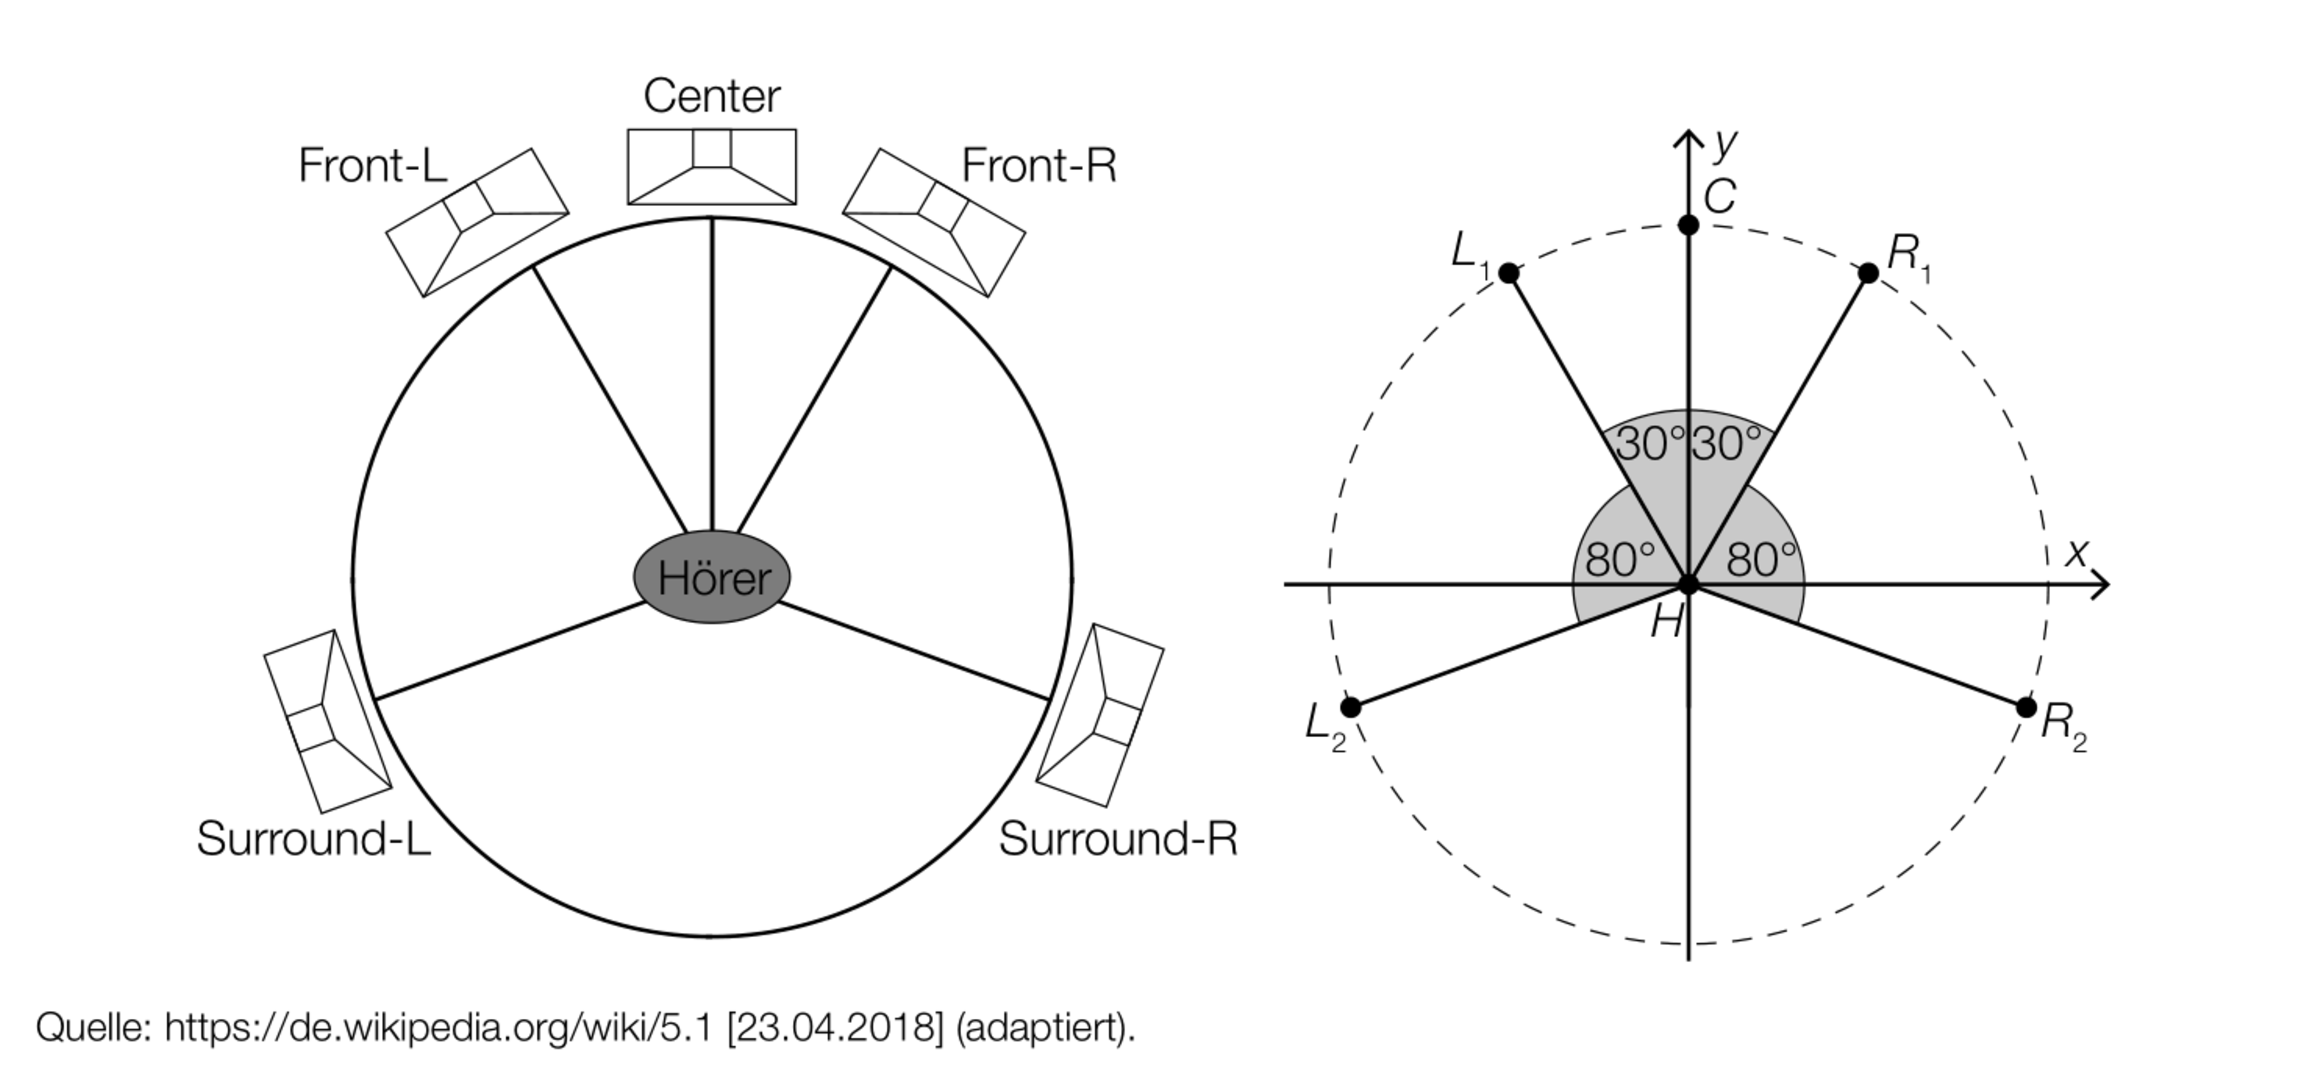
\includegraphics{../Bilder/Bild94-1.eps}}
		\end{center}
		
		Jeder der fünf Lautsprecher $(C, L_1, L_2, R_1, R_2)$ ist in diesem Fall 2\,m vom Hörer $(H)$ entfernt.\\
		Der Punkt $H$ liegt im Koordinatenursprung.
		
		\item \fbox{A} Gib die kartesischen Koordinaten von $R_1$ an!
		
		Gib die Entfernung zwischen $L_2$ und $R_2$ an!
\end{enumerate}

\antwort{
\begin{enumerate}
	\item \subsection{Lösungserwartung:}
	
$T=\dfrac{2\cdot\pi}{c\cdot\pi} \Rightarrow T=\frac{2}{c}$

Mögliche Vorgehensweise:\\
$T=\dfrac{2\cdot\pi}{2\cdot\pi}=1$\\
$\rho_{\text{eff}}=\sqrt{\dfrac{1}{1}\cdot\displaystyle\int^1_0{\sin^2(2\pi\cdot t)}\,\text{d}t}=\frac{1}{\sqrt{2}} \Rightarrow \rho_{\text{eff}}\approx 0,71$\,Pa

\subsection{Lösungsschlüssel:}
- Ein Ausgleichspunkt für eine korrekte Formel. Äquivalente Formeln sind als richtig zu werten.\\
- Ein Punkt für die Berechnung des richtigen Effektivwerts des Schalldrucks, wobei die Einheit "`Pa"' nicht angeführt sein muss.\\
Toleranzintervall: $[0,7\,\text{Pa}; 0,71\,\text{Pa}]$

\item \subsection{Lösungserwartung:}

$T=4$\,ms

Frequenz von $h\!:\frac{1}{0,004}=250$\,Hz

\subsection{Lösungsschlüssel:}
- Ein Punkt für die Angabe der richtigen Periodenlänge von $h$, wobei die Einheit "`ms"' nicht angeführt sein muss.\\
Toleranzintervall: $[3,9\,\text{ms}; 4,1\,\text{ms}]$
- Ein Punkt für die richtige Lösung.

\item \subsection{Lösungserwartung:}

Amplitude von $h\!:$ ca. 2,9 nach ca. 0,2\,ms

Mögliche Begründung:\\
Die Amplitude von $h$ ist nicht gleich der Summe der Amplituden von $h_1, h_2$ und $h_3$, da die drei Funktionen ihre maximlen Funktionswerte zu unterschiedlichen Zeitpunkten erreichen.


\subsection{Lösungsschlüssel:}
- Ein Punkt für die Angabe der richtigen Amplitude und den richtigen Zeitpunkt, wobei die Einheit "`ms"' nicht angeführt sein muss.\\
Toleranzintervalle: $[2,85; 2,95]$ bzw. $[0,19\,\text{ms}; 0,21\,\text{ms}]$
- Ein Punkt für eine korrekte Begründung.

\item \subsection{Lösungserwartung:}

$R_1=(1\mid\sqrt{3})$

Mögliche Vorgehensweise:\\
$x(R_1)=2\cdot\cos(60^\circ)=2\cdot\frac{1}{2}=1$\\
$y(R_1)=2\cdot\sin(60^\circ)=2\cdot\frac{\sqrt{3}}{2}=\sqrt{3}$

Mögliche Vorgehensweise:\\
Entfernung zwischen $L_2$ und $R_2=2\cdot x(R_2)=2\cdot 2\cdot\cos(20^\circ)\approx 3,76$\,m

\subsection{Lösungsschlüssel:}
- Ein Ausgleichspunkt für die Angabe der richtigen Koordinaten von $R_1$.\\
Toleranzintervall für die $y$-Koordinate: $[1,7; 1,75]$
- Ein Punkt für die Angabe der richtigen Lösung.\\
Toleranzintervall: $[3,7\,\text{m}; 3,8\,\text{m}]$

\end{enumerate}}
\end{langesbeispiel}